%; whizzy chapter
% -initex iniptex -latex platex -format platex -bibtex jbibtex -fmt fmt
% 以上 whizzytex を使用する場合の設定。


%     Tokyo Debian Meeting resources
%     Copyright (C) 2009 Junichi Uekawa

%     This program is free software; you can redistribute it and/or modify
%     it under the terms of the GNU General Public License as published by
%     the Free Software Foundation; either version 2 of the License, or
%     (at your option) any later version.

%     This program is distributed in the hope that it will be useful,
%     but WITHOUT ANY WARRANTY; without even the implied warranty of
%     MERCHANTABILITY or FITNESS FOR A PARTICULAR PURPOSE.  See the
%     GNU General Public License for more details.

%     You should have received a copy of the GNU General Public License
%     along with this program; if not, write to the Free Software
%     Foundation, Inc., 51 Franklin St, Fifth Floor, Boston, MA  02110-1301 USA

%  preview (shell-command (concat "evince " (replace-regexp-in-string "tex$" "pdf"(buffer-file-name)) "&"))
% 画像ファイルを処理するためにはebbを利用してboundingboxを作成。
%(shell-command "cd image200901; ebb *.png")

%%ここからヘッダ開始。

\documentclass[mingoth,a4paper]{jsarticle}
\usepackage{monthlyreport}

% 日付を定義する、毎月変わります。
\newcommand{\debmtgyear}{2009}
\newcommand{\debmtgmonth}{4}
\newcommand{\debmtgdate}{18}
\newcommand{\debmtgnumber}{51}



\begin{document}

\begin{titlepage}
\thispagestyle{empty}

% タイトルページ:編集必要な部分は最初のマクロに飛ばすこと

\vspace*{-2cm}
第\debmtgnumber{}回 東京エリア Debian 勉強会資料

\hspace*{-2.4cm}
\includegraphics[width=210mm]{image200801/2008title.eps}\\
\hfill{}\debmtgyear{}年\debmtgmonth{}月\debmtgdate{}日

\end{titlepage}

\dancersection{Introduction}{上川 純一}

\begin{multicols}{2}
 
 
 今月のDebian勉強会へようこそ。これからDebianの世界にあしを踏み入れると
 いう方も、すでにどっぷりとつかっているという方も、月に一回Debianについ
 て語りませんか?

 Debian勉強会の目的は下記です。

 \begin{itemize}
 \item \underline{Debian Developer} (開発者)の育成。
 \item 日本語での「\underline{開発に関する情報}」を整理してまとめ、アップデートする。
 \item \underline{場}の提供。
 \begin{itemize}
  \item 普段ばらばらな場所にいる人々が face-to-face で出会える場を提供
	する。
  \item Debian のためになることを語る場を提供する。
  \item Debianについて語る場を提供する。
 \end{itemize}
 \end{itemize}		

 Debianの勉強会ということで究極的には参加者全員がDebian Packageをがりがり
 と作るスーパーハッカーになった姿を妄想しています。情報の共有・活用を通し
 て Debianの今後の能動的な展開への土台として、「場」としての空間を提供す
 るのが目的です。

 2009年の計画は仮です。

 \begin{enumerate}
  \item 新年の企画 (アンサンブル荻窪開催)
  \item OSC Tokyo
  \item VAIO P インストール記録、
	カーネル読書会 ディストリビューション大集合(小林さん)(東京大学?)
  \item Git Handson (岩松)(あんさんぶる荻窪?)
  \item 家Debianサーバ vs 職場のネットワーク(千代田区都立図書館?\footnote{\url{http://www.library.chiyoda.tokyo.jp/}})
  \item Asterisk (東京大学?)
  \item スペインにて開催
  \item Debconf報告会
  \item OSC Fall?
  \item udev + HAL(岩松さん)
  \item 3D graphics 開発(藤沢さん) 
  \item Debian サーバ+VMware + 各種OS、
	他の仮想化ツール(vserver etc.)、
	忘年会
 \end{enumerate}

 会場候補としては下記があります:

 \begin{itemize}
  \item 大学
  \item 恵比寿SGIホール
  \item Googleオフィス
  \item 公民館(あんさんぶる荻窪等)
  \item 都立会議室(無線LAN)
  \item 健保の施設
 \end{itemize}

\end{multicols}


\newpage

\begin{minipage}[b]{0.2\hsize}
 \definecolor{titleback}{gray}{0.9}
 \colorbox{titleback}{\rotatebox{90}{\fontsize{80}{80} {\gt デビアン勉強会} }}
\end{minipage}
\begin{minipage}[b]{0.8\hsize}
\hrule
\vspace{2mm}
\hrule
%
% there are too many entries in 200901, usually
% we have tocdepth=2.
%
\setcounter{tocdepth}{1}
\tableofcontents
\vspace{2mm}
\hrule
\end{minipage}

\dancersection{事前課題}{上川 純一}

事前課題は:

\begin{enumerate}
 \item 各自の「私のDebian開発ワークフロー」を紹介してください。
\end{enumerate}

この課題に対して提出いただいた内容は以下です。

\begin{multicols}{2}
%; whizzy-master ../debianmeetingresume200904.tex
% $B0J>e$N@_Dj$r$7$F$$$k$?$a!"$3$N%U%!%$%k$G(B M-x whizzytex $B$9$k$H!"(Bwhizzytex$B$,MxMQ$G$-$^$9!#(B

\begin{prework}{$B>e@n=c0l(B}
\preworksection{$B;d$N(BDebian$B%o!<%/%U%m!<(B}

$B%P%0%l%]!<%H$rFI$s$G$+$i(B($B0J2<N,(B)

\preworksection{$B$3$&2~A1$7$?$$(B}

$BA4%"!<%-%F%/%A%c$G$N%S%k%I$H%F%9%H$r<+F02=$7$?$$!#(B

\end{prework}

\begin{prework}{$B$^$($@$3$&$X$$(B}
\preworksection{$B;d$N(BDebian$B%o!<%/%U%m!<(B}

ganttproject$B$r=i$a$F(BITP$B$7$F$+$i;_$^$C$?$^$^!#(B

\preworksection{$B$3$&2~A1$7$?$$(B}

$B2HDm$H;E;v$K1F6A$5$l$:$K%Q%C%1!<%8%a%s%F%J%s%9$G$-$k$h$&$K$7$F$$$-$?$$!#(B

\end{prework}


% \begin{prework}{$BL>A0(B}
% \preworksection{$B;d$N(BDebian$B%o!<%/%U%m!<(B}
% \preworksection{$B$3$&2~A1$7$?$$(B}
% \end{prework}
% $B0J2<$KF1MM$N%F%s%W%l!<%H$GDI2C$9$k!#(B


\begin{prework}{$B>.@n?-0lO:(B}
\preworksection{$B;d$N:n6H4D6-$K$D$$$F(B}
$B2q<R$G$O(B Ubuntu 8.04.1 Desktop $B$r%$%s%9%H!<%k$7$?%G%9%/%H%C%W(BPC$B$G!$(B
$B2H$G$O(B Ubuntu 8.10 $B$r%$%s%9%H!<%k$7$?(B Thinkpad X61 $B$r;H$C$F!$(B
$B3+H/$dF|!9$N6HL3$J$I$r$3$J$7$F$$$^$9!%(B
$BA4A3(B Debian $B$8$c$J$$$N$G$9$,!$(BRuby on Rails $B$J$N$G!$(B
Ruby $B$N(B Version $B$,$"$o$J$$$N$G!$(BUbuntu $B;H$C$F$$$^$9!%(B

GW$BCf$K(B Thinkpad $B$K(B Lenny $BF~$l$kM=Dj$G$9!%(B
$B2q<R$N%5!<%P72$b!$(BDebian $B$K$7$?$$$J$H!$$$$m$$$mLO:wCf$G$9!%(B

\end{prework}

\begin{prework}{$B;3K\9@G7(B}
\preworksection{$B;d$N(BDebian$B%o!<%/%U%m!<(B}

$B%Q%C%1!<%82=$7$?$$%=%U%H%&%'%"$r8+$D$1$?$i!"$^$:<+J,<+?HMQ$NLnNI%Q%C%1!<%8$r:n$j!";n$7$^$9!#<!$KBg;(GD$K%i%$%;%s%9$r3NG'$7!"NI$5$2$J$i!"<+J,$K3e$rF~$l$k$?$a(B ITP $B$7$^$9(B($B>P(B)$B!#$=$l$+$i%3!<%I$J$I!"5;=QE*$J8!F$$KF~$j$^$9(B ($B$3$3$G:C@^$7$?$b$N$b$$$/$D$"$k$N$d$i!D(B)$B!#$5$i$K%3%T!<%i%$%H$d%i%$%;%s%9$N@:::$r$7!"(Bdebian/copyright $B$r40@.$5$;$^$9!#<!$K;d$K$H$C$F$H$F$bFq4X$N(B($B>P(B)$B1Q8l$N%I%-%e%a%s%H$r$D$1$F!"(Bpbuilder $B$G%S%k%I$7$^$9!#:G8e$K(B mentors.debian.net $B$X$N%"%C%W%m!<%I$H(B mentors@org ML$B!"$*$h$S(B debian-develop@jp ML $B$K%a!<%k$rEj$2$F%9%]%s%5!<C5$7$r$7$^$9!#0J>e!#(B

\preworksection{$B$3$&2~A1$7$?$$(B}

$B$_$s$J$,;H$C$F$$$kJ8;z%3!<%I$d(B locale $B$r(B UTF-8 $B$KE}0l$7$?$$!#(B

\end{prework}


\end{multicols}

% image200904/prework.tex 内部にテキストを追加してください。
%
%

\dancersection{最近のDebian関連のミーティング報告}{上川 純一}
\subsection{東京エリアDebian勉強会50回目報告}
% (query-replace-regexp "<.*?>" "")
% (query-replace-regexp "^[	 ]\+" "")

東京エリアDebian勉強会報告。2009年3月21日土曜日に東京エリアDebian勉強会の
第50回を東京大学にて開催しました。

今回の参加者は
岩松, あけど, 前田,キタハラ,たかはし,キタムラ,じつかた,やまだたくま,
日比野,藤澤とおる,よしの,虎,こたに,matsuu,かい,
たなか,ささき(uwabami),
まとはら,こう,John,よしだ@板橋,藤澤りそう,上川x2
の24名でした。

今回事前課題はなかったので参加者の自己紹介をかねて今回に期待することを紹
介してもらいました。関西や新潟から参加している人もいてビックリです。(内容
については発表資料参照)

最初に久しぶりにクイズをしました。9問の簡単な常識問題でした。やまだたくま
さんが全問正解しました。

最近のイベントの紹介をしました。

藤澤とおるさんが gxp と MC-MPI のパッケージ作成について発表しました。パッ
ケージになれてない人がパッケージの作成をしていろいろひっかかった内容を発
表しているのをみながらみんなでにやにや。

日比野さんが common lisp の話をしました。Debian のパッケージでなぜcommon
lisp のライブラリの取扱いがこうなっているのかということを common lisp の
マクロの仕組みから解き明かすセッションでした。素晴らしい。とりあえず
emacsユーザはsbclとslimeのインストールからはじめればよいようです。

最後に今回の期待についておさらいをして、その後に次回の内容を検討しました。
次回はJohnがclozurecl のパッケージ作成したよ、藤澤さんがパッケージを
Debian official にするまでの道、やまねさんがワークフローをさらすので「俺
の開発効率をあげてください」というセッションの三本立ての予定です。

宴会は東京大学の赤門前の宴会場「鉄板焼き 郷」で。

%============================================================
%%% trivia quiz
\dancersection{Debian Trivia Quiz}{上川 純一}

ところで、みなさん Debian 関連の話題においついていますか?Debian関連の話
題はメーリングリストをよんでいると追跡できます。ただよんでいるだけではは
りあいがないので、理解度のテストをします。特に一人だけでは意味がわからな
いところもあるかも知れません。みんなで一緒に読んでみましょう。

今回の出題範囲は\url{debian-devel-announce@lists.debian.org} に投稿された
内容とDebian Project Newsからです。

\begin{multicols}{2}
 %; whizzy-master ../debianmeetingresume200904.tex
% $B0J>e$N@_Dj$r$7$F$$$k$?$a!"$3$N%U%!%$%k$G(B M-x whizzytex $B$9$k$H!"(Bwhizzytex$B$,MxMQ$G$-$^$9!#(B

 \santaku
 {4$B7n(B9$BF|$K%"%C%W%G!<%H$5$l$?(B etch $B$N%P!<%8%g%s$O(B?}
 {4.0r8}
 {4.0beta8}
 {etch-a-sketch}
 {A}
{}

 \santaku
 {4$B7n(B11$BF|$K%"%C%W%G!<%H$5$l$?(B lenny $B$N%P!<%8%g%s$O(B?}
 {5.0r1}
 {5.0.1}
 {lenny++}
 {B}
{}

 \santaku
 {Debian.org DPL $B$K$J$C$?$N$O!)(B}
 {Stefano Zacchiroli}
 {Steve McIntyre}
 {Nobuhiro Iwamatsu}
 {B}
{}

 \santaku
 {Debian JP Leader $B$K$J$C$?$N$O(B?}
 {Kei Hibino}
 {Hiroyuki Yamamoto}
 {Nobuhiro Iwamatsu}
 {C}
{}

 \santaku
 {Debian $B$G?7$7$/DI2C$5$l$?%"!<%-%F%/%A%c$O!)(B}
 {GNU/kFreeBSD i386/amd64}
 {GNU/kMinix-3.0 i386/amd64}
 {GNU/kOpenDarwin i386/amd64}
 {A}
{}

\end{multicols}

% ===============================================================
\dancersection{Java ポリシーを読んでみた}{まえだこうへい}
\index{java policy}
% ===============================================================

\subsection{Java ポリシーを読むハメになった経緯}

初っ端からブチまけると、実はJava ポリシーなんて読むつもりは毛頭なかったのです。なぜなら私は Java なんて大嫌いだからです。長たらしいクラス名やメソッド名なんてみると、身の毛もよだちます。ちゃんと80バイトの幅に収めろよ、って感じです。(わら

冗談\footnote{嫌いなのは本当なんですが。}はさておき、なぜ読むことになったかと言うと、実は別の目的がありました。典型的な手段が目的になってしまった例です。ことの発端は、友人と別件での活動で進捗管理が必要になったためです。某所のPCはadmin権限が与えられておらず、好き勝手にソフトウェアを入れられません。ですが、プロジェクト管理用にGanttProject\footnote{\url{http://www.ganttproject.biz/}}はライセンス使用料無しで導入できるので、これで管理するか、ということにしました。オープンソースソフトウェアなので、きっとDebianにもパッケージがあるに違いない、と。WBSを作り、自宅でDebianにGanttProjectを導入しようとしたら、パッケージが無いではありませんか。使えないとせっかく作ったWBSも更新できず困ります。そこで仕方ないので、ITPしてみることにしました。ちょうど、まだBTSへ投げたことも、ITPもしたことがなく、ある意味ちょうど良いきっかけなのでITPしてみました\footnote{\url{http://bugs.debian.org/cgi-bin/bugreport.cgi?bug=436792}}。

で、Debian Hack Cafeで、岩松さんから「どうせならJava Policy読んで、勉強会のネタにしる」と言われた訳です。特に断る理由もなかったので、やることにしてみました。が、ちょうど今回のDebian勉強会と、KVMの記事\footnote{\url{http://www.atmarkit.co.jp/flinux/rensai/kvm02/kvm02a.html}}の公開が時期的に重なってしまったため、締切り直前で勉強会資料の作成をやっています。終わるのかな。当日の事前配布資料に、このネタが掲載されていればきっと間に合ったのでしょう。

ちなみに、肝心の当初の目的ですが、完全に置いてけぼりを喰らっています。Javaポリシーの翻訳はもう少しで終わるのですが、ITPしたGanttProjectのdebパッケージ化は未着手、GanttProjectで進捗管理する対象は友人が中心に進めているもの、進捗は遅れ気味になっています。巻き返ししなければ。


\subsection{さて、今回の本題。}
前置きが長くなりましたが、今回の本題は、Javaポリシーについて調査してみたよ、でした。要約によれば、背景説明、ポリシーの内容、議論すべき問題点、Javaパッケージメンテナ向けのアドバイスであり、Java仮想マシン、Javaコンパイラ、Javaプログラム、Javaライブラリをターゲットにしています。以下、各章ごとに要点をまとめてみました。

\subsection{1章 背景説明}
要点は2つです。
\begin{itemize}
\item 特定の議題をより詳細に決める場合、Debianポリシーにはサブポリシーとして扱われる。
\item コメントなどをするには、java-commonパッケージチームや、Debian Javaメーリングリストに投稿しる。
\end{itemize}
要は、Javaには固有の事情があるので、Javaポリシーというサブポリシーで扱っているよ、ということです。

\subsection{2章 ポリシー}
Javaパッケージに対するポリシーをまとめています。そのポリシーとは以下のものです。
\begin{itemize}
\item コンパイラ、仮想マシン、ランタイム用の仮想パッケージが作られます。
\item 全Javaコードは、Javaバイトコードとして、全アーキテクチャ向けに配布しなければなりません。
\item 開発者向け(ライブラリ)とエンドユーザ向け(プログラム)の2つのカテゴリに分類されます。
\end{itemize}

\subsubsection{仮想マシン}
Java仮想マシンをパッケージ化する際のポリシーです。パッケージ名、依存関係、コマンド名を規定してます。
\begin{itemize}
\item java-virtual-machineパッケージを提供し、java-commonパッケージに依存していなければなりません。
\item ランタイム環境を配布することもできます。
\item Java2に準拠したランタイムをパッケージでは、java2-runtimeを提供すべきです。\footnote{Java1.1の場合は、java1-runtimeなのですが、今時Java1.1はないと思われるので省略。}
\item Sun Javaプログラムと互換性のあるコマンドラインであれば、/etc/alternatives/javaという名前にするべきです。
\item 必要なランタイム環境を、あらかじめCLASSPATHに設定しておくべきです。
\item JDKのようにコンパイラや仮想マシンのソースコードを提供する場合は、コンパイラパッケージをxxxx-devと命名しなさい。
\item Javaクラスの実装は、ネイティブ言語を用いた処理系で、実行時にロードされる動的ライブラリとしてコンパイルされ、配置されています。仮想マシンがネイティブコードをサポートする場合は、動的ライブラリの検索パスに/usr/lib/jniディレクトリを設定しないといけません。
\end{itemize}

\subsubsection{コンパイラ}
Javaコンパイラに関するポリシーです。仮想マシンの時と基本的には同じで、3点挙げられています。
\begin{itemize}
\item java2-compilerパッケージを提供し、java-commonパッケージに依存していなければなりません。
\item Sun JDKのjavacと互換性があるなら、/etc/alternatives/javacという名前にすべきです。
\item コンパイルに必要なjavaコアクラスをCLASSPATHに設定しておくべきです。
\end{itemize}

\subsubsection{Javaプログラム}
Javaのプログラムに関するポリシーです。
\begin{itemize}
\item /usr/bin以下に配置し、実行可能でなければなりません。
\item プログラムはbinfmt\_miscを使用したJavaクラスか、あるいはラッパーでも構いません。
\item 特定の環境変数\footnote{例えば、CLASSPATHなど}がなくても、実行できなければなりません。
\item 実行ファイルに関するポリシールールに従う必要があります。
\item プログラム自体が補助クラスの場合は、/usr/share/javaディレクトリ配下にjarファイルとして配置しなければなりません。
\item プログラム自体は仮想マシン(java-virtual-machine)とランタイム環境(java2-runtime)に依存していなければなりません。
\item プログラムの名前規則は無く、ユーザ視点で一般的なプログラムです。
\end{itemize}

\subsubsection{Java ライブラリ}
Javaライブラリに関するポリシーです。Javaならではで特徴的なことは、開発者向け\footnote{-devがパッケージ名につくもの。}やユーザ向けのバージョンには分かれていないという点です。

\begin{itemize}
\item Javaでは開発者向けとユーザ向けとでライブラリのバージョンを分けませ
      ん。意味がないからです。
\item Javaライブラリパッケージは、libXXX[version]-javaという形式の名前でなければ
      なりません。
\item version部分はオプションで、必要な部分だけを含むべきです。
\item version部分は名前の衝突を避けるようにすべきです。
\item XXXは実際のパッケージ名です。
\item jarアーカイブのクラスは、/usr/share/java配下に配置しなければなりま
      せん。
\item 名前はpackage[-extraname]-fullversion.jarの形式です。
\item extranameはオプションで、パッケージで提供されているjarとは別に分け
      るためにパッケージ内部で使われます。
\item fullversionはjarファイルのバージョンです。パッケージとは同一ではな
      い場合があります。
\item Javaライブラリはランタイム環境には依存しなければなりませんが、仮想
      マシンには依存すべきではありません。
\end{itemize}
など。

\subsubsection{main, contrib, non-free}
main, contrib, non-freeに分類するためのポリシーです。

\begin{itemize}
\item ソースパッケージがnon-freeなツールでしか(正しく)コンパイルできないなら\footnote{自由なJavaコンパイラは、guavacと、gcjとjikesだけのようです}、mainにすることはできません。パッケージ自体が自由であるなら、contribに入れなければなりません。
\item バイナリパッケージがnon-freeの仮想マシンだけで動くことができるなら\footnote{GNU-Classpathには、自由なバージョンがリストされてます。}、mainにすることはできません。 パッケージ自体が自由であるなら、contribにしなければなりません。
\end{itemize}

\subsection{議論すべき問題}
現在、8つほどの問題が取り上げられています。いずれも議論の余地があるとのことです。
\begin{itemize}
\item リポジトリの名前と存在について。最新バージョンでは削除されています。
\item /usr/share/javaにおけるシンボリックリンクをC言語のライブラリのようにスクリプトで置き換えるべきか否か。
\item コアクラスの必要性について。
\item Sunのコミュニティーソースライセンスは、Debianでは使えるのか?使う場合はどうすれば良いのか\\item すべてのjarファイルは適切なCLASSPATHドキュメントが必要です。
\end{itemize}
以下、省略。


\subsection{Javaパッケージ作成者向けのアドバイス}
Javaパッケージ作成者向けのアドバイス、とはなっているものの、実際のところは、足りないツールを作ってくれだとか、他の言語向けパッケージ作成では自動で行っている部分を手動でやれ、といった話になっています。しかもひどいことに、「これはアドバイスに過ぎず、ポリシーの一部ではない」と言っています。

\begin{itemize}
\item debian/controlのすべての依存関係を手動で管理しなければなりません。Debianの開発ツールではJavaのプログラムを検出することができません。
\item だから、Perlのようにdh\_javaプログラムを作ってくれるボランティアは大歓迎とのこと。
\item debian/rulesの中の、dh\_stripやdh\_shlibdepsのようなJavaには無意味なコマンドを無効にしましょう。
\end{itemize}
などです。

\subsection{まとめ}
実は、ポリシーマニュアルをちゃんと読んだことがまだないので、通常のポリシー
に比べた場合の、Javaポリシーの特徴がどうなのかがよく分かりません。ただ、
自由なコンパイラが3つあるとか、mainに入れるための制約とか、命名規約やら、
依存関係についてのポリシーがあることを知りました。これを元に途中で止まっていたganttprojectのdebパッケージ化を進めます。またプロセスは、本来の目的を達成するために早く進めなきゃです。ついでに、今回訳した文章は、取り合えずdebian-docに投げて査読してもらおうと思います。


\subsection{今月のヨメ八苦}
最近は、毎週水曜のHack Cafeは認めてもらえるようになりました。まあ、本人もその時間にジムに行けるからという理由もありますが。しかし、IRC会議やDebian勉強会以外で、Debian絡みの作業したり、外にでかけると、「またDebian?」と怪訝な顔をされます…。なかなか思うとおりにはならんものです。


% ===============================================================
\dancersection{ocamlに入門してみた}{上川純一}
\index{ocaml}
% ===============================================================

\subsection{ocaml 入門の動機}

ocaml はフランス界隈で流行っている言語のようです。advi や unison などのか
ゆいところに手が届く感じのソフトウェアがocamlで実装されていて、気にはなっ
ていました。ocaml は素晴らしい計算機理論を活用して最新の何かが実装されて
いるという噂は聞いているのですが、いまいち何がどうすごいのかよくわからな
いのでものは試しと、試してみました。

\subsection{ocaml を使うために}

Debian GNU/Linux には ocaml 関連のパッケージが多数入っています。
ためしに検索してみると224パッケージありました。
\begin{commandline}
$ apt-cache search ocaml | wc -l 
224
\end{commandline}

ocamlにはインタラクティブに使うためのインタプリタと、バイナリを生成してく
れるコンパイラの両方があります。ocamlをとりあえず一通り使うためには
ocaml のインタプリタとコンパイラがあればよさそうです。ocaml のネイティブ
コード用のコンパイラは ocaml-native-compilers パッケージのようです。
ocaml のインタープリタは ocaml-interp パッケージのようです。

emacs ユーザとしては、emacs 用のモードも必要です。emacs のモードでそのも
のずばりの ocaml-mode というものもあるのですが、 tuareg というのがよさそ
うなので、それをインストールしてみました。

\begin{commandline}
# apt-get install tuareg-mode ocaml-native-compilers ocaml-interp ocaml
\end{commandline}

\subsection{インタラクティブに使ってみる}

インタラクティブにocamlを使って見ました。
まず足し算をしてみます。

emacs から M-x tuareg-run-caml で ocaml のインタラクティブな端末(ocaml 用語では「トッ
プレベル」という)を起動しました。
足し算をするには、 1 + 2 を入力し、文の終了は ';;' で表現します。

\begin{commandline}
# 1 + 2 ;;
- : int = 3
\end{commandline}

int型の 3 がかえってきました。めでたしめでたし。

\subsection{関数を定義してみる}

では、関数を定義してみます。

\begin{commandline}
# let my_func a b = a + b ;;
val my_func : int -> int -> int = <fun>
# my_func 2 3;;
- : int = 5
\end{commandline}

int int をとって int をかえす関数が定義され、
それを2 と 3 で呼び出したら 5 が帰って来ました。

めでたしめでたし。

型をまったく宣言していないですが、勝手に定義されているあたりが型推論機能
のようです。どうして型が推論できるかということを疑問に思われるかもしれま
せんが、「+」は実は int 専用の足し算です、float の場合は「+.」を使うそう
です。これを知って失神しそうになりました。

\subsection{コンパイルしてみる}

とりあえずインタラクティブに使う方法はわかったので、コンパイルして使う方
法を見てみましょう。ocaml は中間言語に変換する方法とネイティブコンパイル
する方法の二つがあるようです。ocamlcは中間言語、ocamloptはネイティブコン
パイラのようです。ocamlc には二種類のバイナリが提供されており、ocamlc と
ocamlc.opt があります。ややこしいですが、ocamlc.opt はネイティブコンパイ
ラーでコンパイルした中間言語コンパイラーのようです。

\begin{commandline}
$ time ocamlc fibo.ml -o a.1

real	0m0.038s
user	0m0.032s
sys	0m0.004s
$ time ocamlc.opt fibo.ml -o a.2

real	0m0.014s
user	0m0.012s
sys	0m0.000s
\end{commandline}

種類を\tbref{typesofocamlcompilers}にまとめてみました。

\begin{table}[h]
\caption{ocamlコンパイラの種類}
\label{typesofocamlcompilers}
 \begin{tabular}{|c|c|c|}
 \hline
 & ネイティブコンパイルされた & 中間言語にコンパイルされている\\
 \hline
 ネイティブコンパイル結果を出力 &
 ocamlopt.opt & ocamlopt\\
 \hline
 中間言語を出力 &
 ocamlc.opt & ocamlc \\
 \hline
 \end{tabular}
\end{table}


簡単な fibonacci のコードを書いてみて動作速度の雰囲気を感じてみました。
バイトコードのオーバヘッドが感じられる結果になりました。

\begin{commandline}
$ time ./byte-code
102334155

real	0m14.544s
user	0m14.541s
sys	0m0.000s

$ time a./native-code
102334155

real	0m2.933s
user	0m2.932s
sys	0m0.000s
$ time ./fibo.c 40 
102334155

real	0m2.325s
user	0m2.192s
sys	0m0.040s
\end{commandline}


\subsection{ocaml関連のパッケージ化の課題}

Debian パッケージにする際には、コンパイルする回数よりもインストールして
実行される回数のほうが多いため、基本としてはネイティブコンパイルを選択し
ます。
ただし、ネイティブコンパイルできないCPUアーキテクチャもあるため、
どのコンパイラを利用するのかを抽象化するレイヤーが必要です。

ocaml packaging policy によると、ネイティブコンパイラに対応しているのは
amd64, i386, kfreebsd-i386, powerpc, sparc だけだそうです。
重要なアーキテクチャで動きません。たとえば、arm、superh、mipsなどには対
応してないようです。

ライブラリの扱いは特殊で、/usr/lib/ocaml/3.10.2/以下においてあるようです。
ライブラリといっても、バイナリの libxxx.so 共有ライブラリがおいてあるわけではなく、
.mli インタフェースファイルが大量においてあります。
ocamlc -where で発見できるようです。

\begin{commandline}
$ ocamlc -where 
/usr/lib/ocaml/3.10.2
\end{commandline}

ひどい点は、年に一回くらいマイナーバージョンがリリースされているのですが、
その度にライブラリコードがバイナリ非互換に変更されているっぽく、
リビルドするハメになっているようです。

Debian の ocaml メンテナンスチームはあらゆるパッケージを一つのsubversion
リポジトリに統合して管理しているようですが、その理由の一つがこのバージョ
ン間の非互換性ではないでしょうか。

\subsection{参考}
\begin{itemize}
 \item OCaml packaging policy
       \url{http://pkg-ocaml-maint.alioth.debian.org/ocaml_packaging_policy.txt}
 \item dh-ocaml パッケージ
\end{itemize}

\clearpage

%\printindex

\cleartooddpage

\vspace*{15cm}
\hrule
\vspace{2mm}

\includegraphics[width=2cm]{image200502/openlogo-nd.eps}
\noindent \Large \bf Debian 勉強会資料\\ \\
\noindent \normalfont \debmtgyear{}年\debmtgmonth{}月\debmtgdate{}日 \hspace{5mm}  初版第1刷発行\\
\noindent \normalfont 東京エリア Debian 勉強会 (編集・印刷・発行)\\
\hrule


\end{document}
